\section{Introdução}
O Brasil é um dos países mais ricos do mundo em recursos hídricos, facilitando o
desenvolvimento e investimento em geração de energia a partir desse recurso. A
energia hidráulica é a mais dominante em todo o país, e o Brasil é o segundo
país com maior consumo de energia hidrelétrica no mundo com capacidade
instalada de 70.000 MW, 433 usinas hidrelétricas em operação. 

Estima-se que a reforma e melhoria das grandes usinas construídas resultariam
em um aumento potencial de 32.000 MW \citep{goldemberg2007energia},
número que pode ser alcançado, em grande parte, pela manutenção das turbinas
geradoras da energia elétrica. As turbinas estão constantemente expostas aos
fenômenos de abrasão e cavitação, os quais determinam sua vida útil.

O fenômeno de cavitação está muito bem estudado e detalhado em
\cite{escaler2006detection}, onde são apresentadas seus tipos, ocorrências e os
efeitos nas diferentes turbinas. Esse fenômeno físico pode causar erosões na
máquina hidráulica (figura~\ref{fig::cavitacao}), gerando instabilidade de fluxo
de água, vibrações excessivas e redução da eficiência da turbina.

\begin{figure}[h!]
	\centering	
	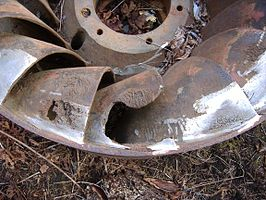
\includegraphics[width=0.7\columnwidth]{sota/figs/intro/cavitacao}
	\caption{Ilustração de uma pá de turbina que sofreu erosão por cavitação.}
	\label{fig::cavitacao}
\end{figure}

A fim de reduzir o desgaste da pá contra cavitação ou abrasão e aumentar a sua
vida útil, utiliza-se a técnica de revestimento por asperção térmica, que pode ser comparada com uma
tinta que protege à exposição com o ambiente. O procedimento é realizado
antes da instalação das pás na turbina por um robô, pois exige alta precisão
e velocidade, além de expelir substâncias nocivas à saúde. Apesar de suficiente para a proteção da pá, o
revestimento também tem vida útil e precisa ser refeito de tempos em tempos para
garantir a proteção da pá contra os fenômenos físicos.

No caso específico da usina hidrelétrica de Jirau, construída no rio Madeira,
os fenômenos de abrasão são intensos devido ao grande número
de partículas que o rio carrega diariamente, reduzindo ainda mais a vida útil do
revestimento.
Portanto, há a necessidade de manutenção regular, o que, na situação atual,
exige paralização da máquina, desmontagem da turbina, posicionamento de cada pá
na área designada ao revestimento, aplicação do revestimento, montagem da
turbina e recalibração. O tempo de paralização para a realização de
toda a manutenção pode levar de um a dois meses, significando uma grande perda
na geração de energia. 

A primeira etapa do projeto EMMA, pesquisa e desenvolvimento
realizados pela Fundação COPPETEC, em parceria com a empresa Rijeza, ANEEL e
ESBR, é um estudo de viabilidade técnica de um sistema robótico para realizar
revestimento por aspersão térmica de turbinas \textit{in situ}, ou seja, dentro
do ambiente da turbina (aro câmara). O projeto tem como objetivo reduzir
significativamente o tempo de manutenção do revestimento por ser realizado no
ambiente confinado da turbina e, portanto, não havendo necessidade de sua
desmontagem.

Este capítulo está dividido da seguinte forma: a seção 2 descreve
detalhadamente o problema, contextualiza o leitor no ambiente da usina de
Jirau e descreve as possíveis tarefas do robô; a seção 3 faz um levantamento do
estado da arte; a seção 4 descreve os projetos conceituais para o robô; e a
seção 5 conclui e descreve os próximos passos para o projeto EMMA. 



